\documentclass[10pt,a4paper,notitlepage]{article}
\usepackage[ngerman,english]{babel}
\usepackage[T1]{fontenc}
\usepackage[utf8]{inputenc}
\usepackage[%right=2cm, left=2.5cm,
 width=16cm,
 bottom=3cm, footskip=1.3cm]{geometry} %A4: 21cm x29,7cm
\usepackage{amsmath}
\usepackage{esdiff}
\usepackage{amsfonts}
\usepackage{amssymb}
\usepackage{graphicx}
\usepackage{booktabs}
\usepackage{tabularx}
\usepackage{caption}
\usepackage{hyperref}
\usepackage{siunitx}
\usepackage{subcaption}
\usepackage{graphicx}
\usepackage{titling}
\usepackage{lipsum} % for filler text
\usepackage{fancyhdr}
\pagestyle{fancy}
\fancyhead{} % clear all header fields
\renewcommand{\headrulewidth}{0pt} % no line in header area
\fancyfoot{} % clear all footer fields
\fancyfoot[LE,RO]{\thepage}           % page number in "outer" position of footer line
\fancyfoot[RE,LO]{h.altug.yildirim@fu-berlin.de - u.kamber@science.ru.nl} % other info in "inner" position of footer line

\fancypagestyle{plain}{%
  \fancyhf{}%
  \fancyfoot[R]{\thepage}%
  \renewcommand{\headrulewidth}{0pt} % no line in header area
  \fancyfoot{} % clear all footer fields
  \fancyfoot[LE,RO]{\thepage}           % page number in "outer" position of footer line
  \fancyfoot[RE,LO]{h.altug.yildirim@fu-berlin.de - u.kamber@science.ru.nl} % other info in "inner" position of footer line
}

\newcommand{\rulesep}{\unskip\ \vrule\ }

\title{Lock-in Amplifier Operation for $dI/dV$ Mapping via Scanning Tunneling Microscopy\vspace{1cm}}

\author{Haydar Altu\u{g} Y{\i}ld{\i}r{\i}m, Umut Kamber}
\begin{document}
\date{24.02.2015}
\maketitle{}
\tableofcontents
\section{Overview}
Usage of lock-in amplifier theory and amplifiers are common in the
experimental science as a measurement technique in noisy environments. Basically, a
reference signal is introduced to an experimental parameter and a filter is used to
extract the signal with same modulation frequency.

In the case of Scanning Tunneling Microscopy (STM) measurements, this
operation is used as a way to map the differential conductivity ($dI/dV$) of the
specimen at a constant energy. In this work we discuss the principal theory behind
this operation.
In the figure \ref{lockin}, the general schematics of the experimental setup can be seen.

\begin{figure}[!ht]
  \centering
  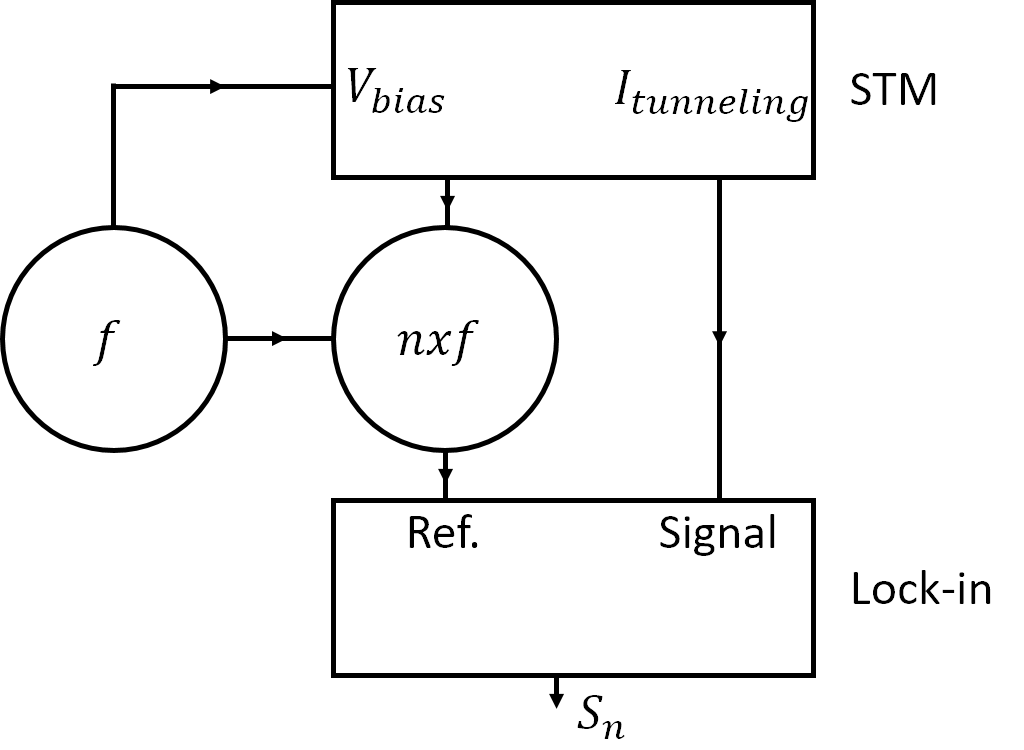
\includegraphics[width=0.4\textwidth]{images/lockin.png}
  \caption{Depiction of the experimental setup with STM and lock-in detection. A wave generator is
used to oscillate the $V_{bias}$ of the system and this cause an oscillation of the $I_{tunneling}$ between the
surface and tip. The lock-in amplifier multiplies this signal with the reference signal coming from the
wave generator to detect the quantity of signal at the exact modulation frequency.}
  \label{lockin}
\end{figure}

\section{Analysis}

In this model we assume our wave generator produce perfect sine wave with the value of $U_0sin(2 \pi ft)$.

\begin{equation}
\label{signal}
\begin{split}
U(t)=V_{bias}+U_0sin(2 \pi ft)
\end{split}
\end{equation}

This signal as equation \ref{signal} suggests, added to $V_{bias}$ . Also it runs through the
lock-in amplifier as a reference signal. It should be noted that the frequency can
contain higher harmonics of the $f$. The $nxf$ indicates this.
In STM, the tunneling current that caused by the quantum tunneling
phenomena is a function of the bias voltage. And with the addition of the driving
signal this $V_{bias}$, it is now become a function time,

\begin{equation}
\label{itunnel}
\begin{split}
I_{tunneling}=I_{tunneling}(V_{bias})=I_{tunneling}(V_{bias}(t))
\end{split}
\end{equation}

It should also be noted that, the signal that run through the lock-in amplifier is
not the $I_{tunneling}$ but the voltage value that converted from $I_{tunneling}$ in the STM
system with an I-V converter.

After two signals fed to the lock-in amplifier, the operation performed. The
operation is basically multiplying the two signal ad then integrated over a longer time
than the periodicity of the signals. The lock-in operation is;

\begin{equation}
\label{liop}
\begin{split}
S_n=\frac{1}{T}\int_{o}^{T} sin(2 \pi ft+\delta \phi)I_{tunneling}(t)dt
\end{split}
\end{equation}

where $T=\frac{m}{f}$, while $m$ is an integer $\gg 1$, indicates relatively long time. And $\delta \phi$ is
phase shift, possibly from different signal path of variables.
In order to perform this operation we need the Taylor expansion of the
$I_{tunneling}$. From Taylor expansion $I_{tunneling}(V_{bias})$ around $U(t=0)=V_{bias}$;

\begin{equation}
\label{}
\begin{split}
I_t(V)=\sum_{\alpha=0}^{\infty}\frac{1}{\alpha!}I^{(\alpha)}(V-V_0)^\alpha \\
I^{(\alpha)}=\left(\left(\frac{\partial}{\partial V}\right)^\alpha I_t\right)_{V=V_0}
\end{split}
\end{equation}

Also we expand the bias voltage as a function of time into its Fourier series to
be able to multiply it with Taylor expansion of the tunneling current to check
orthogonality.

\begin{equation}
  \label{}
  V(t)=\sum_{\mu=0}^{\infty}V_\mu sin(2 \pi f \mu t + \delta \phi_\mu)
\end{equation}

In order to avoid further complications, we will use abbreviation instead of the
sine values;

\begin{equation}
  s_\mu=sin(2 \pi f \mu t+\delta \phi_\mu)
\end{equation}

Then, the Fourier series of the bias voltage is;

\begin{equation}
  V(t)=\sum_{\mu=0}^{\infty} V_\mu s_\mu
\end{equation}

From Taylor expansion;

\begin{equation}
  I(t)=\frac{1}{0!}I(V-V_0)^0+\frac{1}{1!} \left(\frac{\partial I}{\partial V}\right)_{V_0} (V-V_0)^1 +\frac{1}{2!} \left(\frac{\partial^2 I}{\partial V^2}\right)_{V_0} (V-V_0)^2 + \ldots
\end{equation}

And using only the first two harmonics;

\begin{equation}
  V(t)=V_0+V_1 s_1
\end{equation}

The reason that just $\mu=0.1$ cases were used is because we add just one extra
signal to our bias voltage. Even this is not the case the physical parameters mostly
have negligible magnitude at higher harmonics.

If we explicitly write the Taylor expansion of current by taking into account
the voltage;

\begin{equation}
  \label{taylorvoltage}
  \begin{split}
    I(t)=(I)_{V_0}+\left(\frac{\partial I}{\partial V}\right)_{V_0} (V_0+V_1 s_1-V_0) +\frac{1}{2} \left(\frac{\partial^2 I}{\partial V^2}\right)_{V_0} (V_0+V_1 s_1-V_0)^2 \\
    =(I)_{0}+\left(\frac{\partial I}{\partial V}\right)_{V_0} V_1 s_1 +\frac{1}{2} \left(\frac{\partial^2 I}{\partial V^2}\right)_{V_0} {V_1}^2 {s_1}^2
  \end{split}
\end{equation}

From equation \ref{liop} and \ref{taylorvoltage};

\begin{equation}
  \begin{split}
  S_n=\frac{1}{T}\int_{0}^{T}s_1 \left[I_{0}+\left(\frac{\partial I}{\partial V}\right)_{V_0} V_1 s_1 +\frac{1}{2} \left(\frac{\partial^2 I}{\partial V^2}\right)_{V_0} {V_1}^2 {s_1}^2 \right]\partial t \\
  =\frac{1}{T}\int_{0}^{T} \left[I_{0}s_1+\left(\frac{\partial I}{\partial V}\right)_{V_0} V_1 {s_1}^2 +\frac{1}{2} \left(\frac{\partial^2 I}{\partial V^2}\right)_{V_0} {V_1}^2 {s_1}^3 \right]\partial t \\
\end{split}
\end{equation}

We are going to introduce the trigonometric identity in order to evaluate the
sinusoidal multiplications;

\begin{equation}
  sin(x)sin(y)=\frac{1}{2} \left(sin \left(x-y+\frac{\pi}{2}\right)+ sin \left(x+y+\frac{\pi}{2}\right) \right)
\end{equation}

Just consider first two term;

\begin{equation}
  S_n=\frac{1}{T} \int_{0}^{T} \left[I_0 sin\left(2 \pi f t + \delta \phi_1 \right) + \frac{1}{2} \left(\frac{\partial I}{\partial V} \right)_{V_0} V_1 \left(sin \left(\frac{\pi}{2}\right)+sin \left(4 \pi f t + 2 \delta \phi_1 + \frac{\pi}{2} \right) \right) \right] \partial t
\end{equation}

First part of the integral;

\begin{equation}
  \int_{0}^{T} I_0 sin(2 \pi f t + \delta \phi_1) \partial t = \frac{I_0}{2 \pi f} \left(cos(\delta \phi_1)-cos(2 \pi f T + \delta \phi_1) \right)
\end{equation}

And the second part;

\begin{equation}
  \begin{split}
  \frac{1}{2} \int_{0}^{T} \left(\frac{\partial I}{\partial V}\right)_{V_0} V_1 \left(sin\left(\frac{\pi}{2}\right)+sin \left(4 \pi f t +2 \delta \phi_1 +\frac{\pi}{2} \right)\right) \partial t \\
  =\frac{1}{2} \left(\frac{\partial I}{\partial V}\right)_{V_0} V_1 T + \frac{1}{2} \left(\frac{\partial I}{\partial V}\right)_{V_0} V_1 \frac{1}{2 \pi f}\left[cos \left(2 \delta \phi_1 + \frac{\pi}{2}\right)-cos \left(4 \pi f t +2 \delta \phi_1 +\frac{\pi}{2}  \right) \right]
\end{split}
\end{equation}

Thus;

\begin{equation}
  \begin{split}
  S_n=\frac{I_0}{2 \pi f T}\left[cos(\delta \phi_1)-cos(2 \pi f T + \delta \phi_1) \right] + \frac{1}{2} \left(\frac{\partial I}{\partial V}\right)_{V_0} V_1 \\
   + \frac{1}{2} \left(\frac{\partial I}{\partial V}\right)_{V_0} V_1 \frac{1}{2 \pi f T} \left[cos \left(2\delta \phi_1 + \frac{\pi}{2}\right)- cos \left(4 \pi f T + 2\delta \phi_1 + \frac{\pi}{2} \right) \right]
\end{split}
\end{equation}

If initial phase difference is equal to zero $(\delta\phi_1=0)$, and we know $T=\frac{m}{f}$ while $m$ is an integer $\gg 1$;

\begin{equation}
  \begin{split}
  S_n=\frac{I_0}{2 \pi f T}\left[1-cos(2 \pi m) \right] + \frac{1}{2} \left(\frac{\partial I}{\partial V}\right)_{V_0} V_1 \\
   + \frac{1}{2} \left(\frac{\partial I}{\partial V}\right)_{V_0} V_1 \frac{1}{2 \pi f T} \left[cos \left(\frac{\pi}{2}\right)- cos \left(4 \pi m + \frac{\pi}{2} \right) \right]
\end{split}
\end{equation}

\begin{equation}
  \begin{split}
  S_n=\frac{V_1}{2}\left(\frac{\partial I}{\partial V}\right)_{V_0} \left(1-\frac{1}{wT} \right)
\end{split}
\end{equation}

The expression $\left(\frac{\partial I}{\partial V}\right)_{V_0}$ is crucial in here, which is the differential conductivity at constant bias voltage which concludes our efforts.

\section{Acknowledgements}

This work is written under the guidance of the Assoc. Prof. O\u{g}uzhan G\"{u}rl\"{u}.
We used Ralf Vogelgesang’s “Lock-In Amplifier Theory” whitepaper \cite{ralf} extensively as the
main source of this work. We also would like to thank our lab mates at NanoBEEs of Istanbul Technical University for the patience and attention, when we lecture this work.


\bibliographystyle{unsrt}
\bibliography{biblio}

\end{document}
